%碰撞
\documentclass[11pt,tikz,border=3.14mm]{standalone}
\usepackage{pgfplots}
\pgfplotsset{compat=1.17}

\usepackage{xcolor}
\definecolor{r1}{HTML}{FF8674}
\definecolor{b1}{HTML}{17ABDD}
\definecolor{p1}{HTML}{D4B6D6}
\definecolor{g1}{HTML}{70E2CB}
\definecolor{o1}{HTML}{DFA743}

\begin{document}

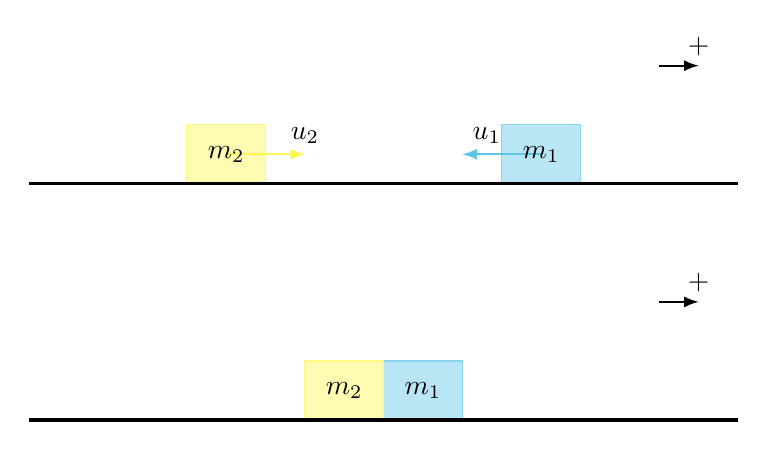
\begin{tikzpicture}
	\begin{scope}
	\draw [fill = b1!30,draw = b1!50] (1,0) rectangle (2,0.75);
	\draw [-latex,b1!70,thick] (1.5,0.375) -- (0.5,0.375) node[above right,black] {$u_{1}$};
	\draw [fill = yellow!30,draw = yellow!50] (-2,0) rectangle (-3,0.75);
	\draw [-latex,yellow!70,thick] (-2.5,0.375) -- (-1.5,0.375) node[ above,black] {$u_{2}$};
	\draw [very thick] (-5,0)--(4,0);
	\draw [-latex,thick] (3,1.5) -- (3.5,1.5) node[above]{+};
	\node at (1.5,0.375) {$m_1$};
	\node at (-2.5,0.375){$m_2$};
	\end{scope}

	\begin{scope}[yshift=-3cm]
	\draw [fill = b1!30,draw = b1!50] (-0.5,0) rectangle (0.5,0.75);
	%\draw [-latex,b1!70,thick] (1.5,0.375) -- (3.5,0.375) node[above right,black] {$v_{1f}$};
	\draw [fill = yellow!30,draw = yellow!50] (-0.5,0) rectangle (-1.5,0.75);
	%\draw [-latex,yellow!70,thick] (-2.5,0.375) -- (-3.5,0.375) node[ above,black] {$v_{2f}$};
	\draw [very thick] (-5,0)--(4,0);
	\draw [-latex,thick] (3,1.5) -- (3.5,1.5) node[above]{+};
	\node at (0,0.375)  {$m_1$};
	\node at (-1,0.375) {$m_2$};
	\end{scope}
\end{tikzpicture}

\end{document}